% !Mode:: "TeX:UTF-8"	% read in as utf8 file.

\chapter{Space beam}
\section{Introduction}
\todo{short introduction}

\section{Displacement model}
Each node of beam element has 6 degrees of freedom, corresponding to 6 nodal forces. For a beam of structure with nodes $ i $ and $ j $, it isshown in figure \ref{fig: space beam element}. \textcolor{red}{In right hand coordinate system}, take x axis as element axis then y and z axes become \textcolor{red}{main moments axes} of cross-section.

\begin{figure}[h!]
\centering
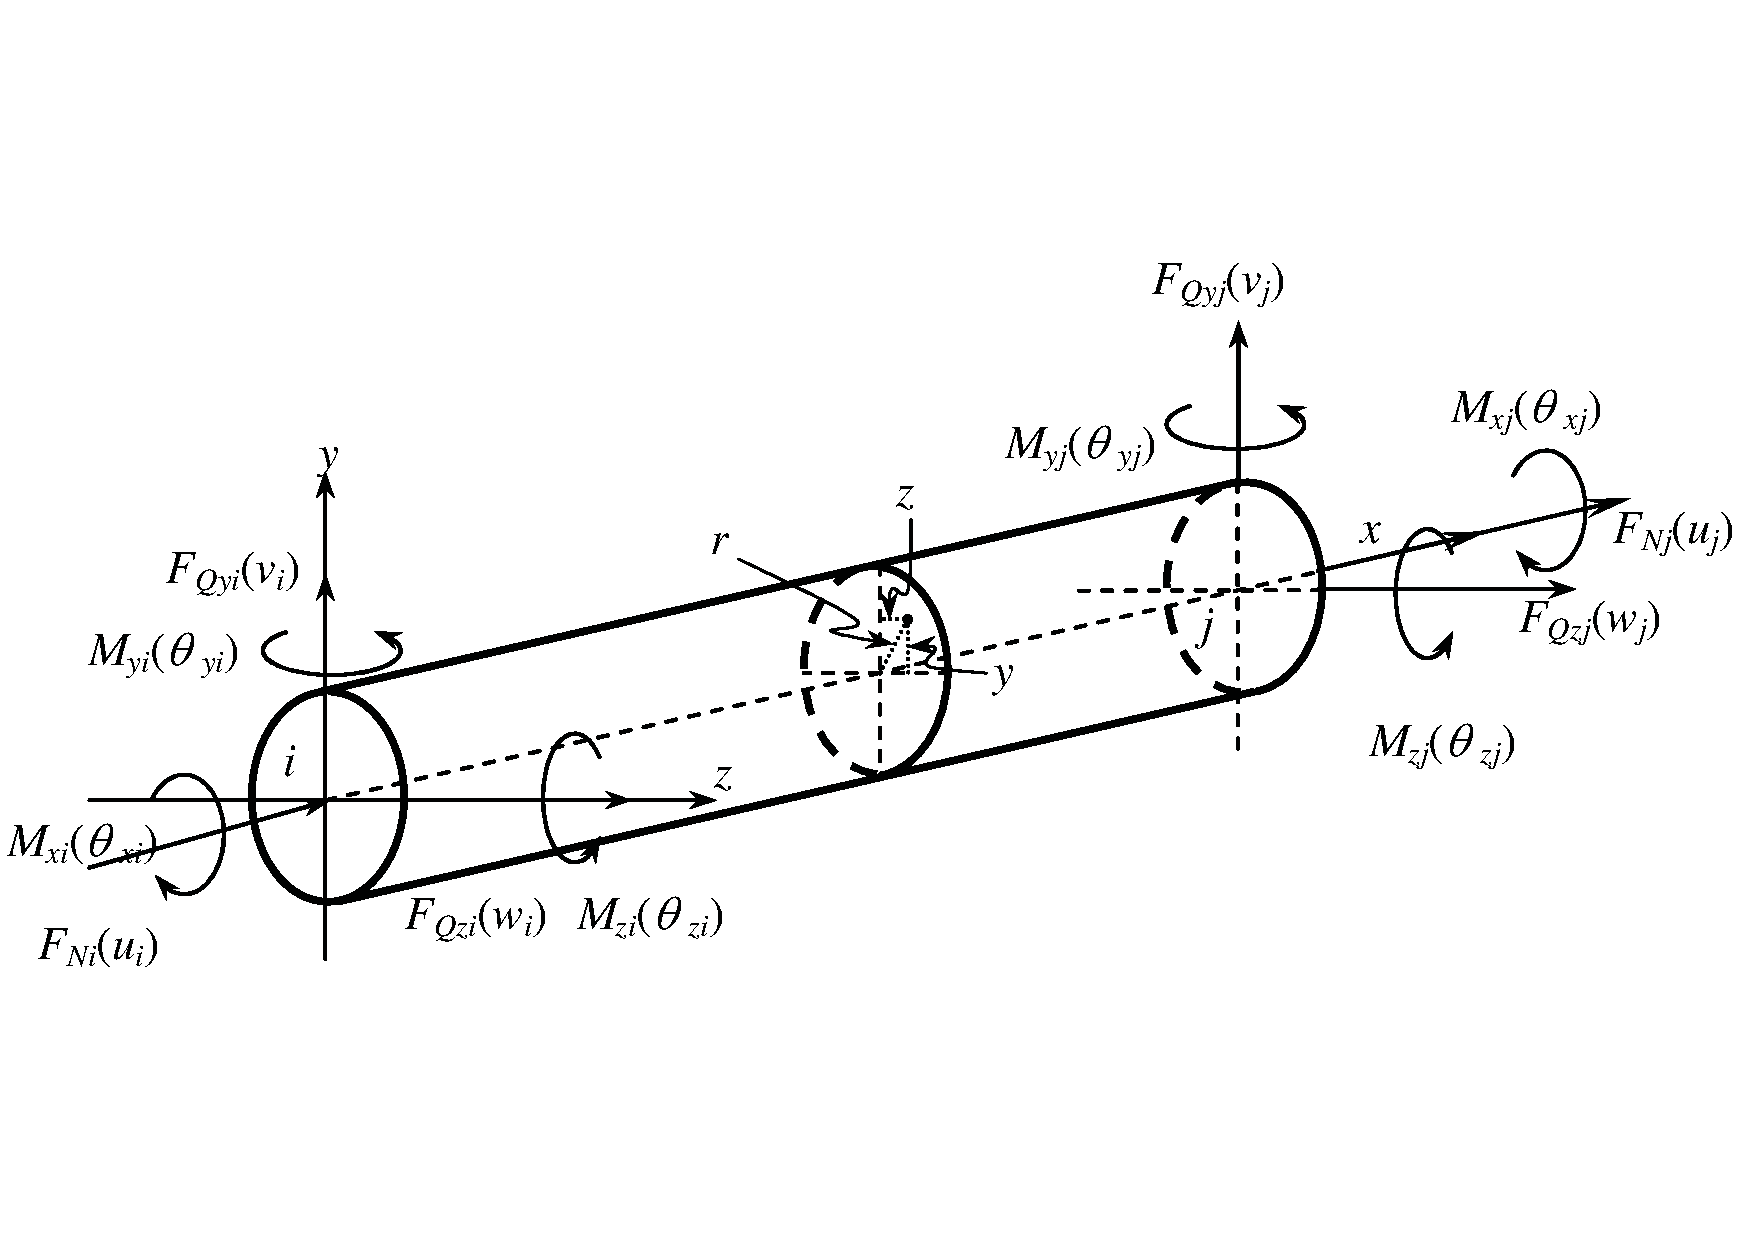
\includegraphics[width=0.5\linewidth]{figure/space_beam_element}
\caption{Beam element}
\label{fig: space beam element}
\end{figure}

The nodal displacements are:

\begin{equation}\label{eq: nodal displacements of beam}
\mathbf{\delta}_i = \begin{bmatrix}
u_i & v_i & w_i & \theta_{xi} & \theta_{yi} & \theta_{zi}
\end{bmatrix} ^T ~~~~ \mathbf{\delta}_j = \begin{bmatrix} u_j & v_j & w_j & \theta_{xj} & \theta_{yj} & \theta_{zj}
\end{bmatrix} ^T
\end{equation}

or simplier:

\begin{equation}\label{key}
\mathbf{\delta}^e = \begin{bmatrix} \mathbf{\delta}_i^T & \mathbf{\delta}_j^T \end{bmatrix}^T
\end{equation}

By assuming a linear interpolation for axial transplacement $ u $ and angular rotation $ \theta_x $, and deflection $ v $ and $ w $ are represented in cubic terms, so we have:

\begin{equation} \label{eq: interpolation scheme for beam element.}
\begin{split} 
	u &= a_0 + a_1 x \\
	v &= b_0 + b_1 x + b_2 x^2 + b_3 x^3 \\
	 w &= c_0 + c_1 x + c_2 x^2 + c_3 x^3 \\
	 \theta_x &= e_0 + e_1 x
\end{split}
\end{equation}

Meanwhile, we can write axial nodal displacements, deflections and rotations in a vector form:

\begin{equation}
\begin{split}
\mathbf{\delta}_u &= \begin{bmatrix} u_i & u_j \end{bmatrix}^T \\
\mathbf{\delta}_v &= \begin{bmatrix} v_i & \theta_{zj} & v_j & \theta_{zj}\end{bmatrix}^T \\
\mathbf{\delta}_w &= \begin{bmatrix} w_i & \theta_{yj} & w_j & \theta_{wj}\end{bmatrix}^T \\
\mathbf{\delta}_\theta &= \begin{bmatrix} \theta_{xi} & \theta_{xj} \end{bmatrix}^T
\end{split}
\end{equation}

Now eq \ref{eq: interpolation scheme for beam element.} becoms:

\begin{equation}\label{key}
u = \mathbf{N}_u \mathbf{\delta}_u ~~~~ \theta_x = \mathbf{N}_\theta \mathbf{\delta}_\theta ~~~~ v = \mathbf{N}_v \mathbf{\delta}_v ~~~~ w = \mathbf{N}_w \mathbf{\delta}_w
\end{equation}

Any displacement inside the element is expressed as:

\begin{equation}\label{eq: displacement inside beam element}
\mathbf{u} = \begin{bmatrix}
u \\ 
v \\ 
w \\ 
\theta_x
\end{bmatrix} = \begin{bmatrix}
\mathbf{H}_u \\ 
\mathbf{H}_v \\ 
\mathbf{H}_w \\ 
\mathbf{H}_\theta
\end{bmatrix} \mathbf{A}^{-1} \mathbf{\delta}^e = \mathbf{N} \mathbf{\delta}^e
\end{equation}

where:

\setcounter{MaxMatrixCols}{20}
\begin{align}
	\mathbf{H}_u(x) &= \begin{bmatrix} 1 & 0 & 0 & 0 & 0 & 0 & x & 0 & 0 & 0 & 0 & 0 \end{bmatrix} \\
	\mathbf{H}_v(x) &= \begin{bmatrix} 0 & 1 & 0 & 0 & 0 & x & 0 & x^2 & 0 & 0 & 0 & x^3 \end{bmatrix} \\
	\mathbf{H}_w(x) &= \begin{bmatrix} 0 & 0 & 1 & 0 & x & 0 & 0 & 0 & x^2 & 0 & x^3 & 0 \end{bmatrix} \\
	\mathbf{H}_\theta(x) &= \begin{bmatrix} 0 & 0 & 0 & 1 & 0 & 0 & 0 & 0 & 0 & x & 0 & 0 \end{bmatrix} 
\end{align}

and 

\begin{equation}\label{key}
A = \begin{bmatrix}
1 & 0 & 0 & 0 & 0 & 0 & 0 & 0 & 0 & 0 & 0 & 0 \\ 
0 & 1 & 0 & 0 & 0 & 0 & 0 & 0 & 0 & 0 & 0 & 0 \\ 
0 & 0 & 1 & 0 & 0 & 0 & 0 & 0 & 0 & 0 & 0 & 0 \\ 
0 & 0 & 0 & 1 & 0 & 0 & 0 & 0 & 0 & 0 & 0 & 0 \\ 
0 & 0 & 0 & 0 & 1 & 0 & 0 & 0 & 0 & 0 & 0 & 0 \\ 
0 & 0 & 0 & 0 & 0 & 1 & 0 & 0 & 0 & 0 & 0 & 0 \\ 
1 & 0 & 0 & 0 & 0 & 0 & l & 0 & 0 & 0 & 0 & 0 \\ 
0 & 1 & 0 & 0 & 0 & l & 0 & l^2 & 0 & 0 & 0 & l^3 \\ 
0 & 0 & 1 & 0 & l & 0 & 0 & 0 & l^2 & 0 & l^3 & 0 \\ 
0 & 0 & 0 & 1 & 0 & 0 & 0 & 0 & 0 & l & 0 & 0 \\ 
0 & 0 & 0 & 0 & 1 & 0 & 0 & 0 & 2l & 0 & 3 l^2 & 0 \\ 
0 & 0 & 0 & 0 & 0 & 1 & 0 & 2 l & 0 & 0 & 0 & 3 l^2
\end{bmatrix} 
\end{equation}

\section{strain and stress}
When beam \textcolor{red}{undergoes tensile, compressional, bending and torsional}  deformation, it's axial strain is composed of three parts: \textcolor{red}{tensile or compressional strain} $ \epsilon_0 $, bending strain $ \epsilon_{by} $ and $ \epsilon_{bz} $. The shear strain caused by torsion is $ \gamma $. Hence,

\begin{equation}\label{key}
\mathbf{\epsilon} = \begin{bmatrix}
\epsilon_0 \\ 
\epsilon_{by} \\ 
\epsilon_{bz} \\ 
\gamma
\end{bmatrix} = \begin{bmatrix}
u' \\ 
-y v'' \\ 
-z w'' \\ 
r \theta_x'
\end{bmatrix} = \begin{bmatrix}
\mathbf{H}_u' \\ 
-y \mathbf{H}_v'' \\ 
-z \mathbf{H}_w'' \\ 
r \mathbf{H}_\theta'
\end{bmatrix} \mathbf{A}^{-1} \mathbf{\delta}^e = \mathbf{B} \mathbf{\delta}^e
\end{equation}

where $ y $ and $ z $ are point in the cross-section, and $ r $ is the distance to $ x $ axis.

By using Hooke's law, the stress can be expressed:

\begin{equation}\label{key}
\mathbf{\sigma} = \begin{bmatrix}
\sigma_0 \\ 
\sigma_{by} \\ 
\sigma_{bz} \\ 
\tau
\end{bmatrix} = \begin{bmatrix}
E\mathbf{H}_u' \\ 
-Ey \mathbf{H}_v'' \\ 
-Ez \mathbf{H}_w'' \\ 
Gr \mathbf{H}_\theta'
\end{bmatrix} \mathbf{A}^{-1} \mathbf{\delta}^e = \mathbf{DB} \mathbf{\delta}^e
\end{equation}

where 

\begin{equation}\label{key}
\mathbf{D} = \mathrm{diag}(E,E,EG)
\end{equation}

\section{stiffness matrix}
The stiffness matrix now can be integrated expressively:

\begin{equation} \label{eq: element stiffness for constant beam}
\begin{split}
\mathbf{K}^e &= \iint dA \int_{0}^{l} \mathbf{B}^T \mathbf{DB} dx \\
&= \begin{bmatrix}
\frac{EA}{l} & 0 & 0 & 0 & 0 & 0 & -\frac{EA}{l} & 0 & 0 & 0 & 0 & 0 \\ 
0 & \frac{12 E I_z}{l^3} & 0 & 0 & 0 & \frac{6 E I_z}{l^2} & 0 & -\frac{12 E I_z}{l^3} & 0 & 0 & 0 & \frac{6 E I_z}{l^2} \\ 
0 & 0 & \frac{12 E I_y}{l^3} & 0 & \frac{6 E I_y}{l^2} & 0 & 0 & 0 & -\frac{12 E I_y}{l^3} & 0 & \frac{6 E I_y}{l^2} & 0 \\ 
0 & 0 & 0 & \frac{G J_k}{l} & 0 & 0 & 0 & 0 & 0 & -\frac{G J_k}{l} & 0 & 0 \\ 
0 & 0 & \frac{6 E I_y}{l^2} & 0 & \frac{4 E I_y}{l} & 0 & 0 & 0 & -\frac{6 E I_y}{l^2} & 0 & \frac{2 E I_y}{l} & 0 \\ 
0 & \frac{6 E I_z}{l^2} & 0 & 0 & 0 & \frac{4 E I_z}{l} & 0 & -\frac{6 E I_z}{l^2} & 0 & 0 & 0 & \frac{2 E I_z}{l} \\ 
-\frac{EA}{l} & 0 & 0 & 0 & 0 & 0 & \frac{E A}{l} & 0 & 0 & 0 & 0 & 0 \\ 
0 & -\frac{12 E I_z}{l^3} & 0 & 0 & 0 & -\frac{6 E I_z}{l^2} & 0 & \frac{12 E I_z}{l^3} & 0 & 0 & 0 & -\frac{6 E I_z}{l^2} \\ 
0 & 0 & -\frac{12 E I_y}{l^3} & 0 & -\frac{6 E I_y}{l^2} & 0 & 0 & 0 & \frac{12 E I_y}{l^3} & 0 & -\frac{6 E I_y}{l^2} & 0 \\ 
0 & 0 & 0 & -\frac{G J_k}{l} & 0 & 0 & 0 & 0 & 0 & \frac{G J_k}{l} & 0 & 0 \\ 
0 & 0 & \frac{6 E I_y}{l^2} & 0 & \frac{2 E I_y}{l} & 0 & 0 & 0 & -\frac{6 E I_y}{l^2} & 0 & \frac{4 E I_y}{l} & 0 \\ 
0 & \frac{6 E I_z}{l^2} & 0 & 0 & 0 & \frac{2 E I_z}{l} & 0 & -\frac{6 E I_z}{l^2} & 0 & 0 & 0 & \frac{4 E I_z}{l}
\end{bmatrix} 
\end{split}
\end{equation} 

In eq \ref{eq: element stiffness for constant beam}, $ I_y = \iint z^2 dA $ and $ I_z = \iint y^2 dA $ are \textcolor{red}{main moments of beam cross-section} with respect to $ y $ and $ z $ axes respectively, $ J_k $ is second area moments about $ x $ axis.

\section{Transformation matrix}

\begin{figure}[h!]
\centering
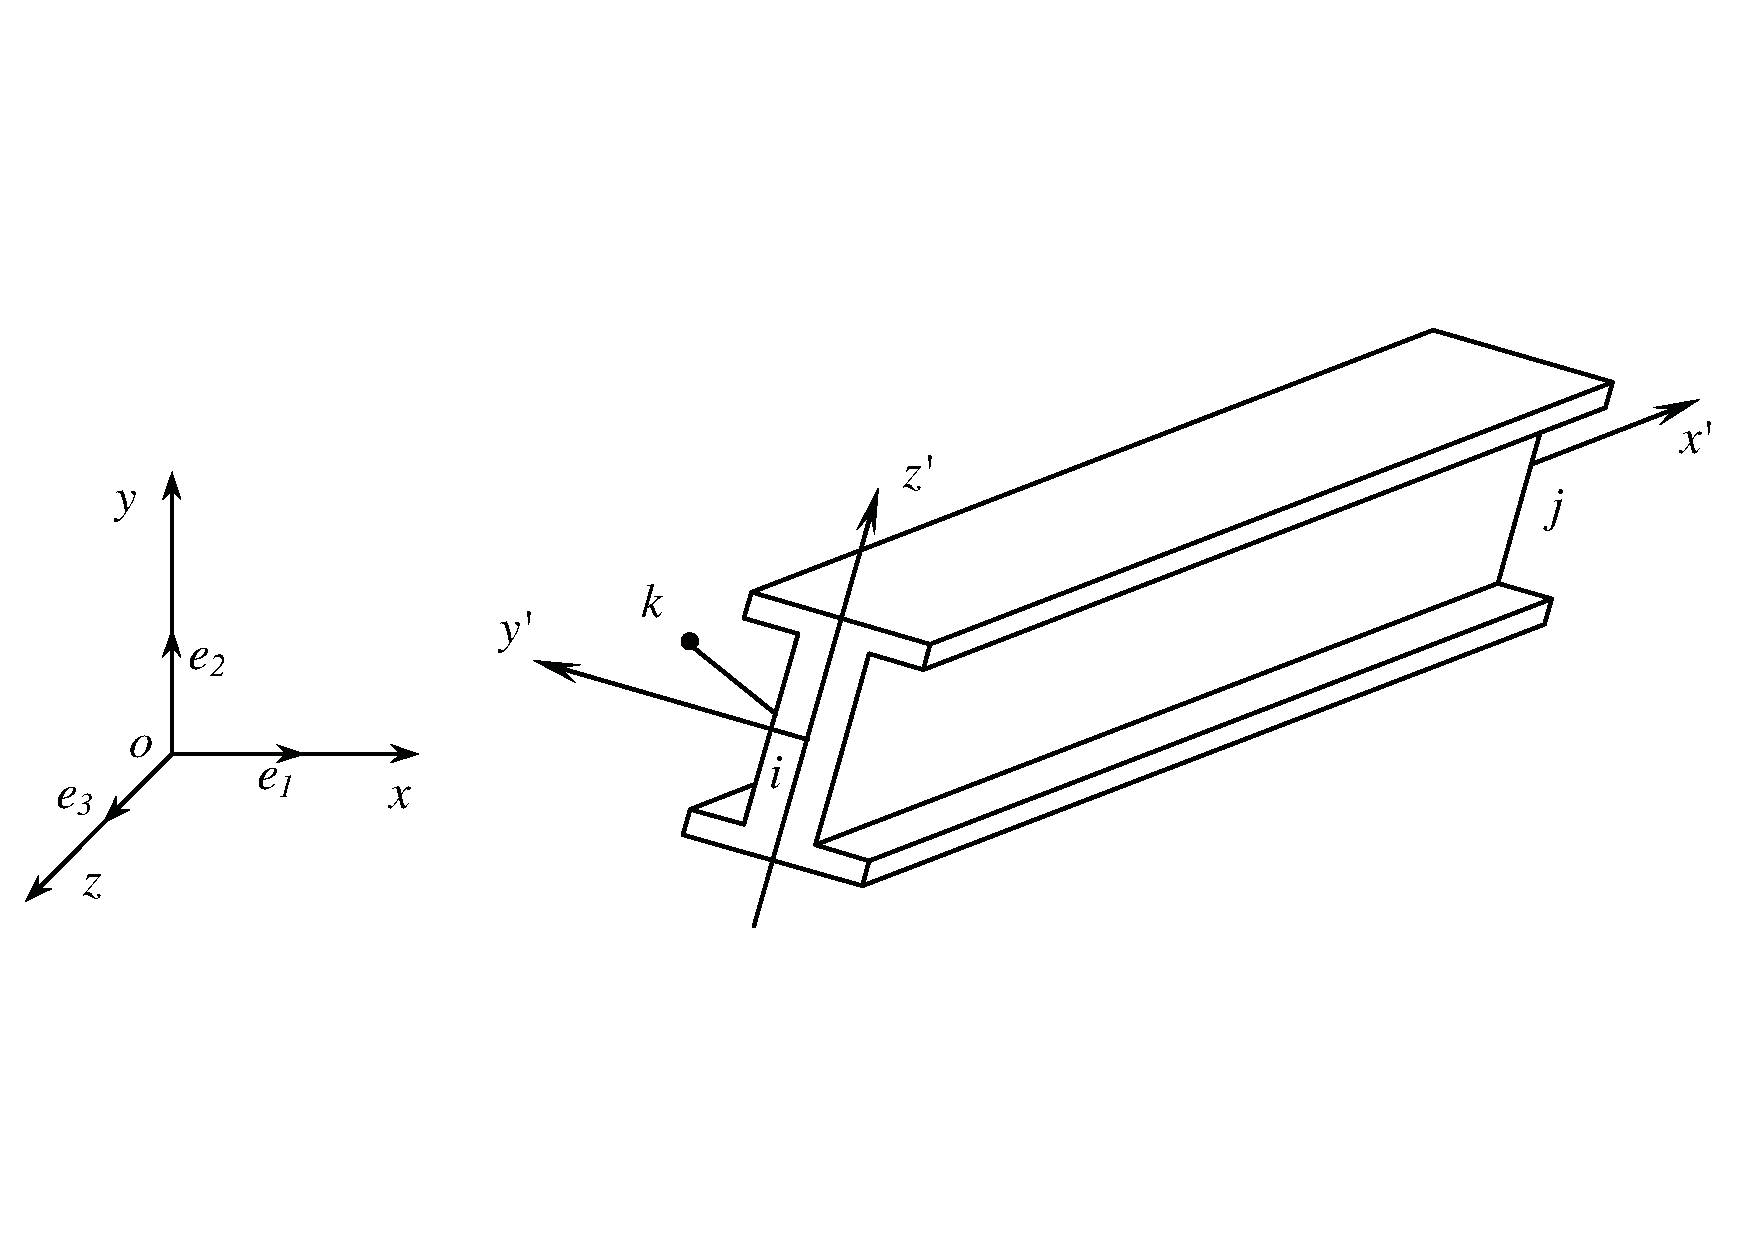
\includegraphics[width=0.5\linewidth]{figure/transformation_for_beam}
\caption{transformation matrix}
\label{fig:transformationforbeam}
\end{figure}

\section{variable beam cross-section... to be added}